\section{環境構築}
\subsection{ローカルでの環境構築}
\TeX でコンパイルを行うためには, TeX Liveをインストールする必要がある.
本書執筆時点(\today 現在)では, TeX Live 2024が最新バージョンであるため,
ここでは, TeX Live 2024のインストール方法を紹介する.
\subsection{TeX Live 2024のインストール}
% Windowsでのインストール方法を簡単に述べる. 
% \begin{enumerate}
%   \item インターネットに置いてあるTeX Liveのインストールファイルをダウンロードする. 
%   \item TeX Liveをインストールする. 
%   \item Visual Studio Codeの拡張機能をインストールする. 
%   \item Visual Studio Codeの設定をしてVS CodeからTeXを使えるようにする. 
% \end{enumerate}
\subsubsection{Windowsの場合}
\url{https://mirror.ctan.org/systems/texlive/tlnet/install-tl-windows.exe}からインストールファイルをダウンロードする.
ダウンロードが終わったら, エクスプローラを開き, \texttt{install-tl-windows.exe}を起動する. このとき,
ファイル名を\textbf{右クリック}して「管理者として実行」をクリックすると, 全てのユーザ向けにインストールする
ことができるため, 必要に応じて管理者権限で実行すると良い. \\
exeファイルを実行すると, 次のようなウィンドウが立ち上がる. デフォルトでinstallが選ばれているので,
installにチェックを入れたまま「Next >」をクリックする. 次のウィンドウでもそのまま「Install」を押せば,
インストールが開始される. なお, この作業は非常に時間がかかるため, 注意が必要.
\begin{figure}[htbp]
  \centering
  \begin{minipage}[b]{.49\textwidth}
    \centering
    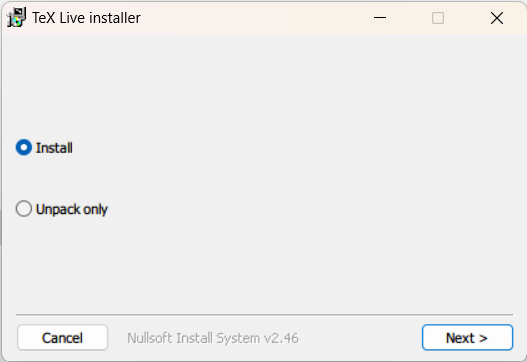
\includegraphics[width=\linewidth]{src/install_windows_1.png}
    \caption{インストールウィンドウ(Windows)(1)}
    \label{fig:ins_win_1}
  \end{minipage}%
  \hspace{.01\textwidth}
  \begin{minipage}[b]{.49\textwidth}
    \centering
    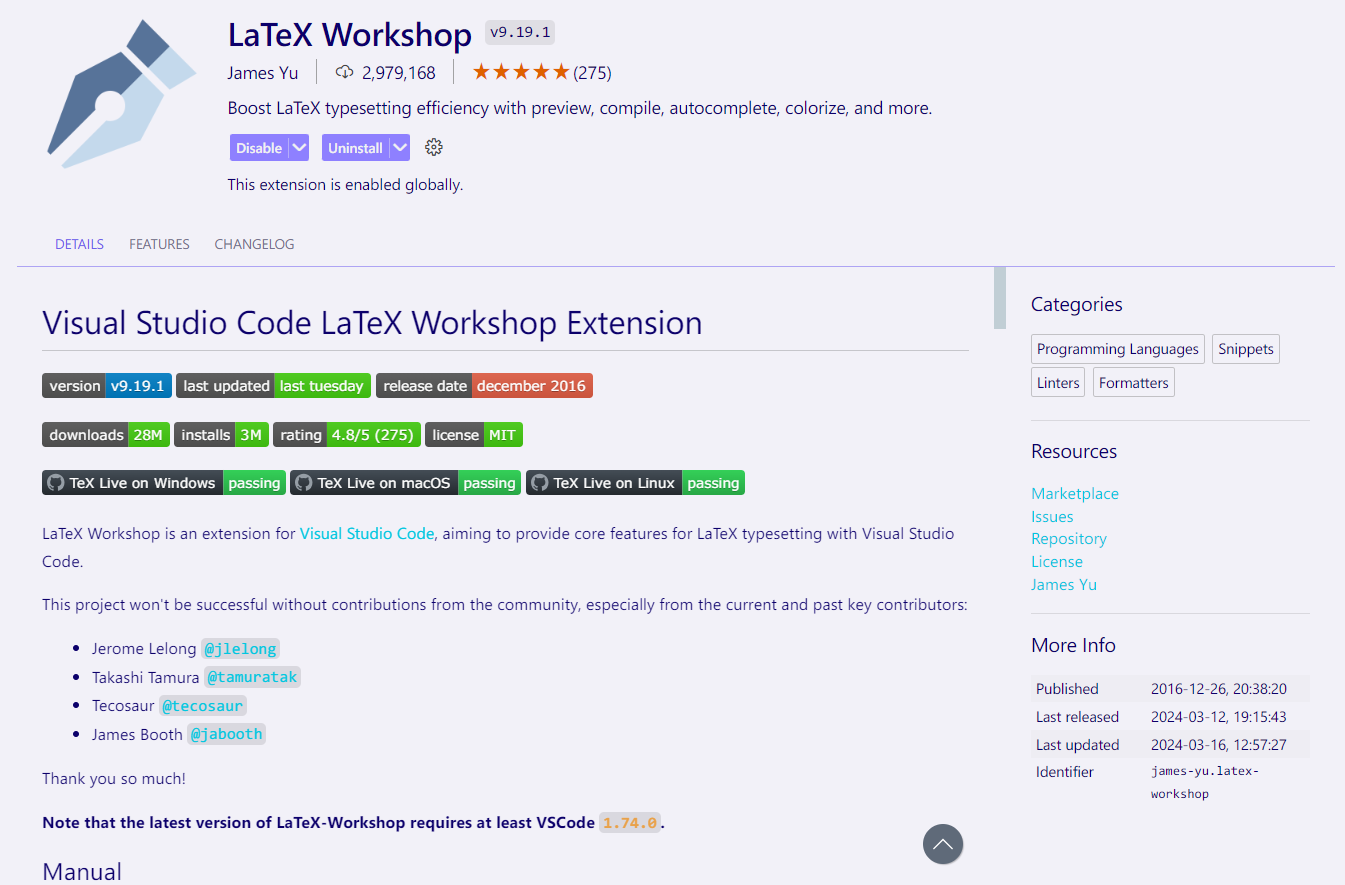
\includegraphics[width=\linewidth]{src/install_windows_2.png}
    \caption{LaTeX Workshop拡張機能}
    \label{fig:ins_win_2}
  \end{minipage}
\end{figure}

\subsubsection{Linux (Ubuntu)の場合}
Linuxでは,流れとしてはWindowsでのインストール方法と大差は無いが,基本的に
コンソール上ですべての工程を行う.
まず,ミラーサイトから\texttt{instal-tl-unx.tar.gz}をダウンロードする必要があるので,
wgetまたはcurlコマンドを使用する.\\
wgetコマンドの場合は,\\
\texttt{wget http://mirror.ctan.org/systems/texlive/tlnet/install\\-tl-unx.tar.gz}\\
curlコマンドの場合は.\\
\texttt{curl -OL http://mirror.ctan.org/systems/texlive/tlnet/install-tl-unx.tar.gz}\\
このコマンドを実行したら,次はダウンロードしたインストーラのファイルを展開する.\\
\texttt{tar xvf install-unx.tar.gz}\\
展開したインストーラのディレクトリに移動する.\\
\texttt{cd install-tl-2*}\\
root権限でインストーラを実行する.\\
\texttt{sudo /install-tl -no-gui -repository \\
  http://mirror.ctan.org/systems/texlive/tlnet/}\\
この時,以下のような表示が出るので,Iを入力してインストールを開始する.
\texttt{
  Actions: \\
  <I> start  installation to hard disk\\
  <H> help\\
  <Q> quit\\
  \\
  Enter command:
}\\
インストールが終了したら/usr/local/binディレクトリは以下にシンボリックリンクを追加する.\\
\texttt{sudo /usr/local/texlive/????/bin/*/tlmgr path add}\\
途中の?や*はワイルドカード検索のため,自動的にうまく実行されるはずだが,そうでない場合は以下の
ように具体的なディレクトリ名を指定する.
\texttt{sudo /usr/local/texlive/2024/bin/x86\_64-linux/tlmgr path add}\\
もし以上の解説でうまくいかない場合は,TeXWikiのインストールガイド(\url{https://texwiki.texjp.org/?Linux})を参照してほしい.

\subsubsection{Mac OSの場合}
Mac OSでは,Mac向けのTeX LiveのパッケージであるMacTeXの導入が推奨されている.
基本的にはフルインストールを推奨するので,以下にフルインストールのためのコマンドを紹介する.
\begin{itemize}
  \item GUIアプリケーションありの場合\\
        \noindent
        \texttt{
          brew install --cask mactex\\
          sudo tlmgr update --self --all\\
          sudo tlmgr paper a4
        }
  \item GUIアプリケーションなしの場合\\
        \texttt{
          brew install --cask mactex-no-gui\\
          sudo tlmgr update --self --all\\
          sudo tlmgr paper a4
        }
\end{itemize}
Homebrewが入っていない場合はHomebrew公式HPからダウンロード・インストールすること.\\
Homebrew日本語公式ホームページ: \url{https://brew.sh/ja/}

\subsection{VS CodeにTeXの拡張機能を追加する}
TeX Liveのインストールが終われば, 次はVS Codeから\TeX をコンパイルできるようにする
必要がある. まず, \TeX の拡張機能をインストールしよう. VS Codeの「拡張機能」にて,
「LaTeX Workshop」と検索すれば同名の拡張機能が出てくるため, それをインストールする.
(図\ref{fig:ins_win_2}参照)\\

基本的には以上で作業は完了である.